% Select language used in document (ngerman or english). Automatically
% generated text is translated accordingly.
% use \selectthesislanguage in body.tex to switch to default language

\documentclass[ngerman, paper]{mmt} % use for BA1
%\documentclass[english, bachelorthesis]{mmt} % use for BA2
%\documentclass[ngerman, masterthesis]{mmt} % use for Master thesis

\usepackage{mathptmx}
\usepackage{graphicx}
\usepackage{times}
\usepackage{subfig}
\usepackage{float}
\usepackage[utf8]{inputenc}
\usepackage{listings}
\usepackage{makecell}
\usepackage[anythingbreaks]{breakurl}

\usepackage{amsmath}
\usepackage[autostyle,german=guillemets]{csquotes}

% moved to cls file. use \selectthesislanguage to switch to default language
%\usepackage[english,ngerman]{babel}

\usepackage{abbrevs}
%% the following solves a bug in the abbrevs package, that adds an empty
%% space after the abbrev
\makeatletter
\renewcommand\maybe@space@{%
  % \@tempswatrue % <= this is in the original
  \maybe@ictrue % <= this is new
  \expandafter   \@tfor
    \expandafter \reserved@a
    \expandafter :%
    \expandafter =%
                 \nospacelist
                 \do \t@st@ic
  % \if@tempswa % <= this is in the original
  \ifmaybe@ic % <= this is new
    \space
  \fi
}
\makeatother
%%


\usepackage{listings}
\usepackage{color}
\definecolor{lightgray}{rgb}{.9,.9,.9}
\definecolor{darkgray}{rgb}{.4,.4,.4}
\definecolor{purple}{rgb}{0.65, 0.12, 0.82}
\lstdefinelanguage{JavaScript}{
  keywords={break, case, catch, continue, debugger, default, delete, do, else, false, finally, for, function, if, in, instanceof, new, null, return, switch, this, throw, true, try, typeof, var, let, const, void, while, with},
  morecomment=[l]{//},
  morecomment=[s]{/*}{*/},
  morestring=[b]',
  morestring=[b]",
  ndkeywords={class, export, boolean, throw, implements, import, this},
  keywordstyle=\color{blue}\bfseries,
  ndkeywordstyle=\color{darkgray}\bfseries,
  identifierstyle=\color{black},
  commentstyle=\color{purple}\ttfamily,
  stringstyle=\color{red}\ttfamily,
  sensitive=true
}

\lstset{
   language=JavaScript,
   backgroundcolor=\color{lightgray},
   extendedchars=true,
   basicstyle=\footnotesize\ttfamily,
   showstringspaces=false,
   showspaces=false,
   numbers=left,
   numberstyle=\footnotesize,
   numbersep=9pt,
   tabsize=2,
   breaklines=true,
   showtabs=false,
   captionpos=b
}

\usepackage[authordate,bibencoding=auto,strict,noibid,backend=biber]{biblatex-chicago}
\bibliography{bibliography}

%% Add configuration options
\newabbrev{\authorname}{Vorname Nachname}
\newabbrev{\authormail}{vnachname.mmt-b2015@fh-salzburg.ac.at}
\newabbrev{\titlename}{Titel der Arbeit}
\newabbrev{\advisor}{Titel Vorname Nachname}
%\newabbrev{\secondadvisor}{Titel Vorname Nachname}
\newabbrev{\thesisdate}{dd.mm.yyyy}
\newabbrev{\keywordsenglish}{word1, word2, word3}
\newabbrev{\keywordsgerman}{wort1, wort2, wort3}


%% Paper title.

\title{\titlename}

%% This is how authors are specified in the conference style

%% Author 
\author{ \authorname\\ \scriptsize \authormail \\ \scriptsize 
\ifmmtlanguagegerman FH Salzburg \else Salzburg University of Applied Sciences \fi
}

%% A teaser figure can be included as follows, but is not recommended since
%% the space is now taken up by a full width abstract.
%\teaser{
%  \includegraphics[width=1.5in]{sample.eps}
%  \caption{This can be a teaser image of the thesis.}
%}

%% Abstract section for paper format.
\abstract{
    Lorem ipsum dolor sit amet, consectetur adipiscing elit. Aenean venenatis nulla vestibulum dignissim molestie. Quisque tristique tortor vitae condimentum egestas. Donec vitae odio et quam porta iaculis ut non metus. Sed fermentum mauris non viverra pretium. Nullam id facilisis purus, et aliquet sapien. Pellentesque eros ex, faucibus non finibus a, pellentesque eu nibh. Aenean odio lacus, fermentum eu leo in, dapibus varius dolor. Lorem ipsum dolor sit amet, consectetur adipiscing elit. Proin sit amet ornare velit. Donec sit amet odio eu leo viverra blandit. Ut feugiat justo eget sapien porttitor, sit amet venenatis lacus auctor. Curabitur interdum ligula nec metus sollicitudin vestibulum. Fusce placerat augue eu orci maximus, id interdum tortor efficitur.

}

%%%%%%%%%%%%%%%%%%%%%%%%%%%%%%%%%%%%%%%%%%%%%%%%%%%%%%%%%%%%%%%%
%%%%%%%%%%%%%%%%%%%%%% START OF THE PAPER %%%%%%%%%%%%%%%%%%%%%%
%%%%%%%%%%%%%%%%%%%%%%%%%%%%%%%%%%%%%%%%%%%%%%%%%%%%%%%%%%%%%%%%%

\begin{document}

\selectthesislanguage

\pagenumbering{gobble}

 % group open
\ifmmtpaper 
\begingroup 
    % is required because paper template messes with sizes
    \fontsize{12}{18}\selectfont        
    \setlength{\parindent}{0pt}
    \setlength{\parskip}{5pt plus 2pt minus 1pt}
    \sectionfont{\fontsize{14}{15}\selectfont}
\fi

    \begin{titlepage}

% check if second advisor exists
\newcommand{\printsecondadvisor}[1]{%
  \ifcsname#1\endcsname%
  \ifmmtlanguagegerman ZweitbetreuerIn: \else Second Advisor: \fi \secondadvisor 
  \else%
    
  \fi%
}

\ifmmtmasterthesis

    
    % \begin{center}
    %     \Huge{ 
    %     	\textbf{\ifmmtlanguagegerman Masterarbeit \else Master Thesis \fi}
    %     }
    % \end{center}
    
    \newpage
    
    \thispagestyle{empty}
    
    \hfill 
\includegraphics[height=1.5cm]{images/FHSLogo.jpg}
    
    \vspace*{2cm}
    
    \Large{
    \titlename
    
    \vspace*{1cm}
    
    \ifmmtlanguagegerman
    Masterarbeit zur Erlangung des akademischen Grades
    \else
    Master thesis in partial fulfilment of the requirements for\\ the degree of 
    \fi
    
    \vspace*{0.5cm}
    
    \textit{Master of Science}
    }
    
    
    \vspace*{1.5cm}
    {\large
    \ifmmtlanguagegerman AutorIn: \else Author: \fi \authorname
    }
    \vfill
    
    {\normalsize
    \ifmmtlanguagegerman
    Vorgelegt am FH-Masterstudiengang MultiMediaTechnology, Fachhochschule Salzburg
    \else
    Submitted to the Master degree program MultiMediaTechnology, Salzburg University of Applied Sciences
    \fi
    
    
    \vspace*{1cm}
    
    \ifmmtlanguagegerman BetreuerIn: \else Advisor: \fi
    \advisor
    \\    
    \printsecondadvisor{secondadvisor}
    
    \vfill
    
    Salzburg, \ifmmtlanguagegerman Österreich, \else Austria, \fi  \thesisdate
    }

\else % Bachelor thesis title page

    \begin{center}
    
    
\includegraphics[width=5cm]{images/FHSLogo.jpg}


    \vspace*{4cm}
    
    \fontsize{20.79}{18pt}{\selectfont        
    %\Large{
    	\textit{\textbf{\titlename}}
    %}
    }
    
    \vspace*{4cm}
    
    \fontsize{20.79}{18pt}{%\large{
    \ifmmtlanguagegerman
    	\textbf{Bachelorarbeit \ifmmtpaper 1 \else 2 \fi }
    \else
        \textbf{Bachelor Thesis \ifmmtpaper 1 \else 2 \fi }
    \fi
    }
    
    
    \end{center}
    
    \vfill
    
    %\begin{tabular}{ll}
    \ifmmtlanguagegerman AutorIn: \else Author: \fi  \authorname  \\
    \ifmmtlanguagegerman BetreuerIn: \else Advisor: \fi \advisor \\
    \printsecondadvisor{secondadvisor}
    
    Salzburg, \ifmmtlanguagegerman Österreich, \else Austria, \fi \thesisdate
    
    
    
    % uncomment the following 3 lines for an optional lock flag, max. 2 years!
    %\hfill
    %\color{red}
    %\framebox{Sperrvermerk bis 20/01/2012}

\fi

\end{titlepage}
        
    \onecolumn           
    
    \pagenumbering{roman}
    
    \newpage
    
\ifmmtlanguagegerman
\subsection*{Eidesstattliche Erklärung}


Ich erkläre hiermit eidesstattlich, dass  ich  die vorliegende Bachelorarbeit selbständig  und ohne fremde Hilfe verfasst, und keine  anderen  als die angegeben Quellen und  Hilfsmittel benutzt  habe. Weiters versichere ich hiermit, dass ich   die den benutzten Quellen  wörtlich oder inhaltlich entnommenen Stellen als solche kenntlich gemacht habe.

Die Arbeit wurde bisher in gleicher oder ähnlicher Form keiner anderen Prüfungskommission weder im In- noch im Ausland vorgelegt und auch nicht veröffentlicht.

\else

\subsection*{Affidavit}

I herewith declare on oath that I wrote the present master thesis without the help of third persons and without using any other sources and means listed herein; I further declare that I observed the guidelines for scientific work in the quotation of all unprinted sources, printed literature and phrases and concepts taken either word for word or according to meaning from the Internet and that I referenced all sources accordingly.

This thesis has not been submitted as an exam paper of identical or similar form, either in Austria or abroad and corresponds to the paper graded by the assessors.

\fi

\vspace*{3cm}

%{\bf \thesisdate{}}


\hfill

\ifmmtlanguagegerman
$\overline{Datum \hspace{2cm}}$ \hfill $\overline{{Unterschrift}\hspace{3cm}}$

\vspace*{1cm}

\hfill $\overline{{Vorname\hspace{2cm}Nachname}}$
 
 \else
 $\overline{Date \hspace{2cm}}$ \hfill $\overline{{Signature}\hspace{4cm}}$

\vspace*{1cm}

 \hfill $\overline{{First~Name\hspace{2cm}Last~Name}}$
 \fi

  % comment out for expose

% group closing
\ifmmtpaper
\endgroup
\fi

%\ifmmtpaper\else
    
    \newpage
    \selectlanguage{ngerman}
    \section*{Kurzfassung}
    Lorem ipsum dolor sit amet, consectetur adipiscing elit. Aenean venenatis nulla vestibulum dignissim molestie. Quisque tristique tortor vitae condimentum egestas. Donec vitae odio et quam porta iaculis ut non metus. Sed fermentum mauris non viverra pretium. Nullam id facilisis purus, et aliquet sapien. Pellentesque eros ex, faucibus non finibus a, pellentesque eu nibh. Aenean odio lacus, fermentum eu leo in, dapibus varius dolor. Lorem ipsum dolor sit amet, consectetur adipiscing elit. Proin sit amet ornare velit. Donec sit amet odio eu leo viverra blandit. Ut feugiat justo eget sapien porttitor, sit amet venenatis lacus auctor. Curabitur interdum ligula nec metus sollicitudin vestibulum. Fusce placerat augue eu orci maximus, id interdum tortor efficitur.
    
    \ifmmtmasterthesis    
    \vspace*{0.5cm} 
    \textbf{Schlüsselwörter:~} \keywordsgerman
    \fi
    
    \newpage
    \selectlanguage{english}
    \section*{Abstract}
    Lorem ipsum dolor sit amet, consectetur adipiscing elit. Aenean venenatis nulla vestibulum dignissim molestie. Quisque tristique tortor vitae condimentum egestas. Donec vitae odio et quam porta iaculis ut non metus. Sed fermentum mauris non viverra pretium. Nullam id facilisis purus, et aliquet sapien. Pellentesque eros ex, faucibus non finibus a, pellentesque eu nibh. Aenean odio lacus, fermentum eu leo in, dapibus varius dolor. Lorem ipsum dolor sit amet, consectetur adipiscing elit. Proin sit amet ornare velit. Donec sit amet odio eu leo viverra blandit. Ut feugiat justo eget sapien porttitor, sit amet venenatis lacus auctor. Curabitur interdum ligula nec metus sollicitudin vestibulum. Fusce placerat augue eu orci maximus, id interdum tortor efficitur.

    
    \ifmmtmasterthesis        
    \vspace*{0.5cm} 
    \textbf{Keywords:~} \keywordsenglish
    \fi
    
    \selectthesislanguage
    
    \newpage
    \tableofcontents

%\fi

\mmtcolumnmode % switch back to column formatting of stylesheet

\maketitle % used for paper formatting

\ifmmtpaper\else
\pagestyle{headings}
\fi
\pagenumbering{arabic}


%for reference to this section
\section{Einleitung}
\label{section:Introduction}
Einleitungstext......

\section{Formatierung}
\label{section:Formatting}


Text mit beliebigen Sonderzeichen in UTF-8 ohne BOM \ldots
,
\textbf{hervorgehobener Text},
\texttt{void}\footnote{Fußnote 1},
mathematische Formel im Text $\sum_{i=0}^n i^2$
\ldots

Referenz auf Unterabschnitt \ref{subsection:Coding} der Arbeit, automatisch richtig nummeriert.

\textcite[]{Mulloni:2010} bringen einen Literaturverweis im laufenden Text.

Literaturverweise sind essentiell für eine wissenschafliche Arbeit. \autocite[]{McConnell:2004:CCS:1096143}.

Achtung: nur zitierte Literatur wird im Literaturverzeichnis
angeführt.\footnote{Fußnote 2}


Wir verwenden \LaTeX\footnote{ \url{http://en.wikibooks.org/wiki/LaTeX}} -- und das
ist keine Quelle, sondern blos eine URL.

\subsection{Figures machen was sie wollen}

% h = try to place the figure Here
% t = try to place the figure at the Top of a page
% p = try to place this figure along with others on a separate Page
% Note that LaTeX has a sophisticated ranking algorithm to place figures.
% It is not always easy to accept LaTeX's placing but it is harder doing it
% manually. Just let it go ;-)
\begin{figure}[!ht]
	\centering
	\subfloat[Das Julia Fraktal]{
		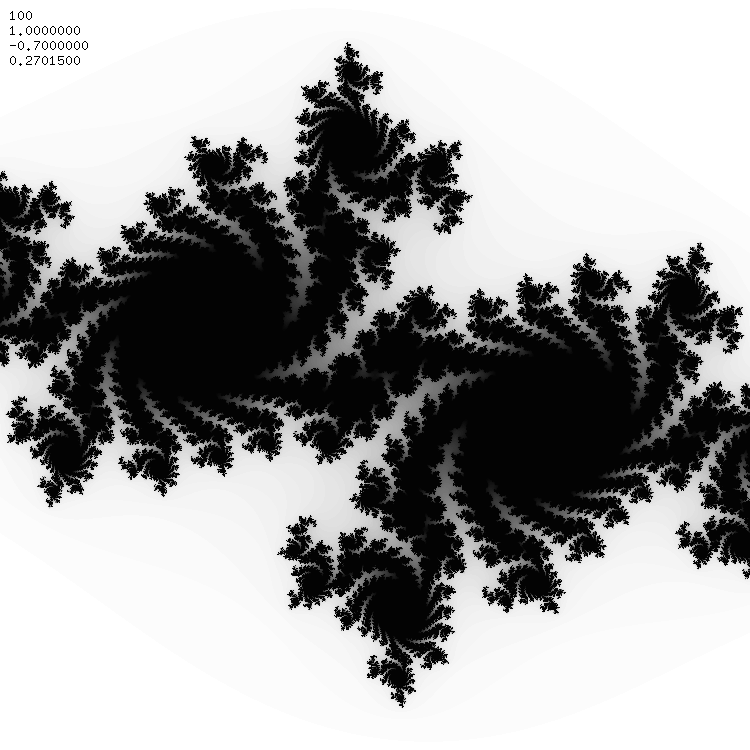
\includegraphics[width=0.75\linewidth]{images/Julia-Fractal.png}
		%for reference of this subfigure only
		\label{subfigure:Julia-Fractal}
	}
	\qquad
	\subfloat[Noise für Tinteneffekte]{
		
\includegraphics[width=0.75\linewidth]{images/Perlin-Coherent.png}
		%for reference of this subfigure only
		\label{subfigure:Perlin-Coherent}
	}
	\caption[
		Verschiedene Pixelgraphiken\newline
		% source url given in the table of figures
		\small\texttt{https://mediacube.at/wiki/}
	]{
		Verschiedene Pixelgraphiken
	}
	%for reference to all subfigures
	\label{figure:PixelImages}
\end{figure}

Unterstützte Pixelgraphikformate: PNG, JPEG, PDF.
Angabe von height oder width meist wichtig.

Referenz auf Abbildung \ref{figure:PixelImages} mit allen Teilbildern.
Referenz auf Unterabbildung \ref{subfigure:Julia-Fractal}.

%figure* stretches figure over both columns
\begin{figure*}[t]
	\centering
	
\includegraphics[width=0.9\textwidth]{images/KappaGamma.pdf}
	\caption{
		Vektorgraphik mit \LaTeX\ Beschriftung ($\kappa$, $\gamma$)
	}
	%for reference to this figure
	\label{figure:KappaGammaTau}
\end{figure*}

Referenz auf Abbildung \ref{figure:KappaGammaTau}.

Bei Vektorgraphik mit \LaTeX\ Beschriftung keine Skalierung mit width
oder height verwenden!
Vektorgraphik mit \LaTeX\ Beschriftung kann etwa mit \texttt{ipe} erstellt
werden.

Unterstütztes Vektorgraphikformat: PDF. EPS muss konvertiert werden.


\subsection{Unterabschnitt 2}
%for references to this subsection
\label{subsection:Coding}

\begin{lstlisting}[
	label=listing:Main, %for reference to this listing
	float=h,
	caption=main.cpp,
	firstnumber=10
]
int main(void) {
	while (true) {
	}
	return 0;
}
\end{lstlisting}

Wie man in Listing \ref{listing:Main} in Zeile 10 sieht, kann man die Zeilennummern im Listing absichtlich setzen, hier z.B. auf 10. In Listing \ref{listing:closure} wurde davon nicht Gebrauch gemacht. In diesem Fall beginnt die Nummerierung bei 1.

\begin{lstlisting}[
    label=listing:closure,
	float=h,
	caption=Closure in Javascript,
	language=JavaScript
]
function foo(x,y) {
    let i = x;
    return function(a) {
        return i * 2;
    }
}
\end{lstlisting}


\subsubsection{Unterunterabschnitt i}

Wörtliches Zitat:
%select proper language if not in German
\selectlanguage{english}
\begin{quote}
``Erwin Unruh discovered that templates can be used to compute
something at compile time. [...] The intriguing part of this exercise, however, was that the production of the prime numbers was performed by the compiler during the compilation process and not at run time.''

\autocite[305]{Bosch2014}
\end{quote}
%select German again or the language that you were using before (note ngerman stands for New German)
%\selectlanguage{ngerman}
\selectthesislanguage


\subsection{Unterabschnitt b}

\begin{enumerate}
	\item Punkt 1
	\begin{enumerate}
		\item Unterpunkt 1
		\item Unterpunkt 2
	\end{enumerate}
	\item Punkt 2
\end{enumerate}

\begin{itemize}
	\item Punkt 1
	\begin{itemize}
		\item Unterpunkt 1
		\item Unterpunkt 2
	\end{itemize}
	\item Punkt 2
\end{itemize}


\subsection{Unterabschnitt c}

\begin{table}[ht]
	\centering
	\begin{tabular}{r|rrr}
		    & $i$ & $j$ & $k$ \\ \hline
		$i$ &$-1$ & $k$ &$-j$ \\
		$j$ &$-k$ &$-1$ & $i$ \\
		$k$ & $j$ &$-i$ &$-1$
	\end{tabular}
	\caption{
		Multiplikationstabelle für Quaternionen
	}
	\label{table:Quaternions}
\end{table}

Referenz auf Tabelle \ref{table:Quaternions}.

\section{Abschnitt 2}
\label{section:MathematicalStuff}

Sei $f(x)$ eine stetige Funktion, so ist die \textbf{Fourier Transformierte}
$F(\omega)$ wie folgt definiert:
\begin{equation}
\label{equation:FourierDefinition}
	F(\omega) = \int_{-\infty}^{\infty} f(x) e^{-i\omega t} dt
\end{equation}

Referenz auf mathematische Gleichung (\ref{equation:FourierDefinition}).

Unnummerierte Gleichung:
\begin{equation*}
	e^{i\varphi} = \cos\varphi + i \sin\varphi
\end{equation*}
%you may also use \[ \] instead of \begin{equation*} and \end{equation*}

Gleichungssystem:
\begin{eqnarray}
	g(x) = f(x - x_0) & \Leftrightarrow &
		G(\omega) = F(\omega) e^{-i\omega x_0} \\
	g(x) = f(x) e^{i\omega_0 x} & \Leftrightarrow &
		G(\omega) = F(\omega - \omega_0)
\end{eqnarray}
 % the main text

%\input{acknowledgements}

%\ifmmtpaper\else % only use the following for thesis format

\newpage
\onecolumn    
\ifmmtlanguagegerman
\section*{Abkürzungsverzeichnis}
\else
\section*{Abbreviations}
\fi

\begin{table}[h]		
	\begin{tabular}{ll}
		TCP & Transmission Control Protocol \\
		VR & Virtual Reality \\			
	\end{tabular}
\end{table}

\listoffigures
\lstlistoflistings
\listoftables

\newpage

%\fi

\printbibliography

 % group open
\ifmmtpaper 
\begingroup 
    % is required because paper template messes with sizes
    \fontsize{12}{18}\selectfont        
    \setlength{\parindent}{0pt}
    \setlength{\parskip}{5pt plus 2pt minus 1pt}
    \sectionfont{\fontsize{14}{15}\selectfont}
\fi

\newpage
\onecolumn
\appendix

\textbf{\color{red} Anhänge löschen, die nicht verwendet werden.}

\section*{Appendix}
\addcontentsline{toc}{section}{Appendices}
\renewcommand{\thesubsection}{\Alph{subsection}}

\subsection{git-Repository}

Das Repository dient zur Dokumentation und Nachvollziehbarkeit der Arbeitsschritte. Stellen Sie sicher, dass der/die BetreuerIn Zugriff auf das Repository hat. Stellen im Sinne des Datenschutzes sicher, dass das Repository nicht für andere zugänglich ist.

Daten für Bachelorarbeit 1 und 2:

\begin{itemize}
	\item LaTeX-Code der finalen Version der Arbeit
	\item alle Publikationen, die als pdf verfügbar sind.
	\item alle Webseiten als pdf
\end{itemize}

Daten für Bachelorarbeit 2:
\begin{itemize}
	\item Quellcode für praktischen Teil
	\item Vorlagen für Studienmaterial (Fragebögen, Einverständniserklärung, ...)	
	\item eingescanntes, ausgefülltes Studienmaterial (Fragebögen, Einverständniserklärung, ...)
	\item Rohdaten und aufbereitete Daten der Evaluierungen (Log-Daten, Tabellen, Graphen, Scripts, ...)	
\end{itemize}

Link zum Repository auf dem MMT-git-Server {\url{gitlab.mediacube.at}:

{\color{red}\url{https://gitlab.mediacube.at/fhs123456/Abschlussarbeiten-Max-Muster}}
	
\subsection{Vorlagen für Studienmaterial}

Vorlagen für Studienmaterial müssen in den Anhang. 

\subsection{Archivierte Webseiten}
% \show\UrlBreaks

\url{http://web.archive.org/web/20160526143921/http://www.gamedev.net/page/resources/_/technical/game-programming/understanding-component-entity-systems-r3013}, letzter Zugriff 1.1.2016

\url{http://web.archive.org/web/20160526144551/http://scottbilas.com/files/2002/gdc_san_jose/game_objects_slides_with_notes.pdf}, letzter Zugriff 1.1.2016




% group closing
\ifmmtpaper
\endgroup
\fi


\end{document}
